Another important type of latent variable models are latent growth curve
models. Growth modeling is often used to analyze longitudinal or
developmental data. In this type of data, an outcome measure is measured
on several occasions, and we want to study the change over time. In many
cases, the trajectory over time can be modeled as a simple linear or
quadratic curve. Random effects are used to capture individual
differences. The random effects are conveniently represented by
(continuous) latent variables, often called \emph{growth factors}. In
the example below, we use an artifical dataset called
\texttt{Demo.growth} where a score (say, a standardized score on a
reading ability scale) is measured on 4 time points. To fit a linear
growth model for these four time points, we need to specify a model with
two latent variables: a random intercept, and a random slope:

\begin{verbatim}
# linear growth model with 4 timepoints
# intercept and slope with fixed coefficients
 i =~ 1*t1 + 1*t2 + 1*t3 + 1*t4
 s =~ 0*t1 + 1*t2 + 2*t3 + 3*t4
\end{verbatim}

In this model, we have fixed all the coefficients of the growth
functions. To fit this model, the lavaan package provides a special
\texttt{growth()} function:

\begin{Shaded}
\begin{Highlighting}[]
\NormalTok{model <-}\StringTok{ ' i =~ 1*t1 + 1*t2 + 1*t3 + 1*t4}
\StringTok{           s =~ 0*t1 + 1*t2 + 2*t3 + 3*t4 '}
\NormalTok{fit <-}\StringTok{ }\KeywordTok{growth}\NormalTok{(model, }\DataTypeTok{data=}\NormalTok{Demo.growth)}
\KeywordTok{summary}\NormalTok{(fit)}
\end{Highlighting}
\end{Shaded}

\begin{verbatim}
lavaan (0.5-13) converged normally after  44 iterations

  Number of observations                           400

  Estimator                                         ML
  Minimum Function Test Statistic                8.069
  Degrees of freedom                                 5
  P-value (Chi-square)                           0.152

Parameter estimates:

  Information                                 Expected
  Standard Errors                             Standard

                   Estimate  Std.err  Z-value  P(>|z|)
Latent variables:
  i =~
    t1                1.000
    t2                1.000
    t3                1.000
    t4                1.000
  s =~
    t1                0.000
    t2                1.000
    t3                2.000
    t4                3.000

Covariances:
  i ~~
    s                 0.618    0.071    8.686    0.000

Intercepts:
    t1                0.000
    t2                0.000
    t3                0.000
    t4                0.000
    i                 0.615    0.077    8.007    0.000
    s                 1.006    0.042   24.076    0.000

Variances:
    t1                0.595    0.086
    t2                0.676    0.061
    t3                0.635    0.072
    t4                0.508    0.124
    i                 1.932    0.173
    s                 0.587    0.052
\end{verbatim}

Technically, the \texttt{growth()} function is almost identical to the
\texttt{sem()} function. But a mean structure is automatically assumed,
and the observed intercepts are fixed to zero by default, while the
latent variable intercepts/means are freely estimated. A slightly more
complex model adds two regressors (\texttt{x1} and \texttt{x2}) that
influence the latent growth factors. In addition, a time-varying
covariate \texttt{c} that influences the outcome measure at the four
time points has been added to the model. A graphical representation of
this model is presented below.

\begin{verbatim}
## Warning: col2rgb(0) is deprecated
\end{verbatim}

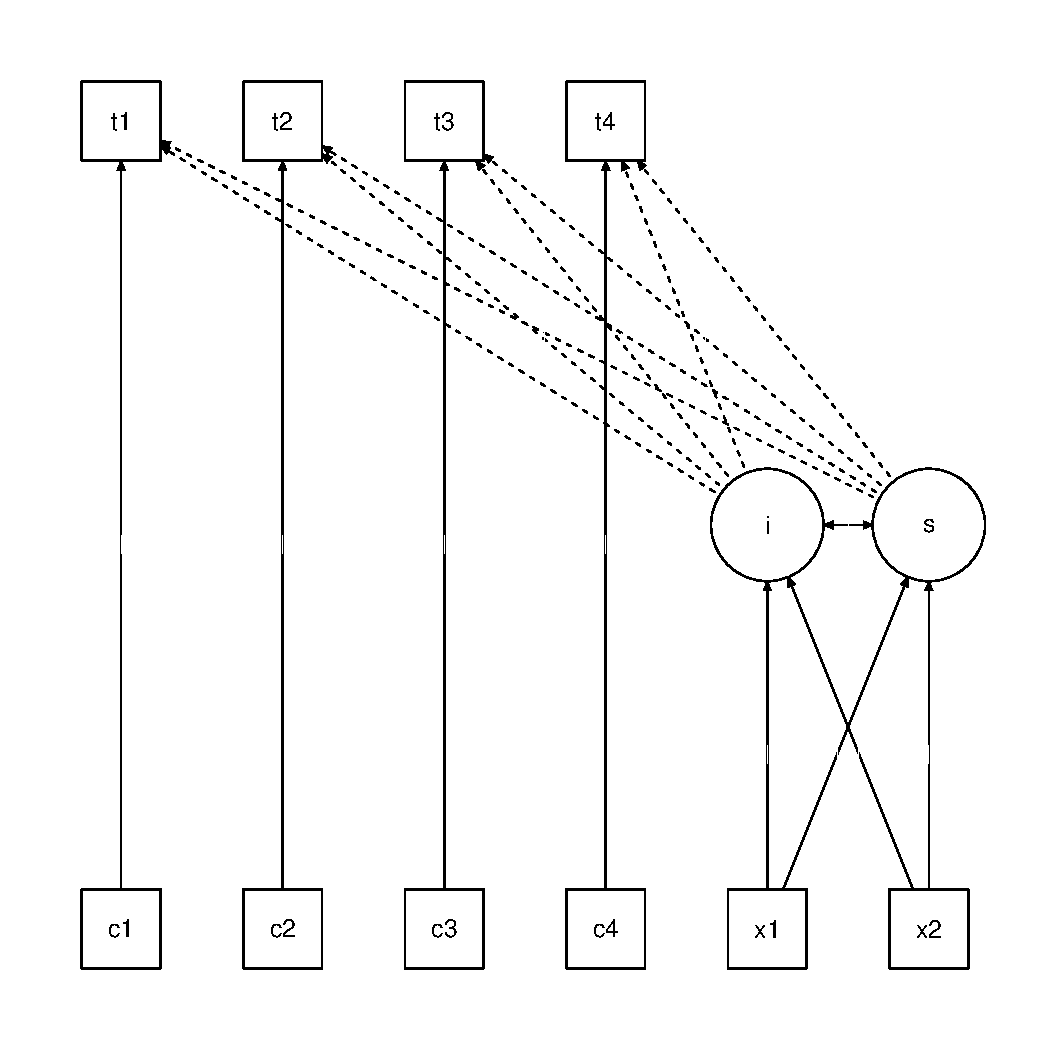
\includegraphics{figure/growth.pdf}

The corresponding syntax is the following:

\begin{verbatim}
# intercept and slope
# with fixed coefficients
  i =~ 1*t1 + 1*t2 + 1*t3 + 1*t4
  s =~ 0*t1 + 1*t2 + 2*t3 + 3*t4
# regressions
  i ~ x1 + x2
  s ~ x1 + x2
# time-varying covariates
  t1 ~ c1
  t2 ~ c2
  t3 ~ c3
  t4 ~ c4
\end{verbatim}

For ease of copy/pasting, the complete R code needed to specify and fit
this linear growth model with a time-varying covariate is printed again
below:

\begin{Shaded}
\begin{Highlighting}[]
\CommentTok{# a linear growth model with a time-varying covariate}
\NormalTok{model <-}\StringTok{ '}
\StringTok{  # intercept and slope with fixed coefficients}
\StringTok{    i =~ 1*t1 + 1*t2 + 1*t3 + 1*t4}
\StringTok{    s =~ 0*t1 + 1*t2 + 2*t3 + 3*t4}
\StringTok{  # regressions}
\StringTok{    i ~ x1 + x2}
\StringTok{    s ~ x1 + x2}
\StringTok{  # time-varying covariates}
\StringTok{    t1 ~ c1}
\StringTok{    t2 ~ c2}
\StringTok{    t3 ~ c3}
\StringTok{    t4 ~ c4}
\StringTok{'}
\NormalTok{fit <-}\StringTok{ }\KeywordTok{growth}\NormalTok{(model, }\DataTypeTok{data =} \NormalTok{Demo.growth)}
\KeywordTok{summary}\NormalTok{(fit)}
\end{Highlighting}
\end{Shaded}

